% Created 2023-10-24 mar 23:11
% Intended LaTeX compiler: pdflatex
\documentclass[11pt]{article}
\usepackage[utf8]{inputenc}
\usepackage[T1]{fontenc}
\usepackage{graphicx}
\usepackage{grffile}
\usepackage{longtable}
\usepackage{wrapfig}
\usepackage{rotating}
\usepackage[normalem]{ulem}
\usepackage{amsmath}
\usepackage{textcomp}
\usepackage{amssymb}
\usepackage{capt-of}
\usepackage{hyperref}
\usepackage{../modern}
\bibliography{./fuentes.bib}
\raggedbottom
\setcounter{secnumdepth}{2}
\author{Luis Eduardo Galindo Amaya (1274895)}
\date{16 de Octubre 2023}
\title{Taller 6. Procesos}
\hypersetup{
 pdfauthor={Luis Eduardo Galindo Amaya (1274895)},
 pdftitle={Taller 6. Procesos},
 pdfkeywords={},
 pdfsubject={},
 pdfcreator={Emacs 27.1 (Org mode 9.3)}, 
 pdflang={Spanish}}
\begin{document}

\modentitlepage{../images/escudo-uabc-2022-1-tinta-pos.png}
\tableofcontents\pagebreak
\datasection{Individual}

\section{Introduccion}
\label{sec:orgdf7bf91}
A lo largo de esta practica aprenderemos que son los procesos dentro del los 
sistemas operativos, como funcionan para que sirven y como podemos utilizarlos 
de manera efectiva para lograr diversos tipos de tareas. 
\pagebreak

\section{Desarollo}
\label{sec:org78f6ccd}
\subsection{Genere un listado completo de todos los procesos que están en el sistema y muestre la información completa de todos los que se empezaron a ejecutar el 7 de septiembre en una sola línea.}
\label{sec:orga1d15be}

\begin{verbatim}
ps -ef | grep "Sep 7"
\end{verbatim}

\begin{figure}[htbp]
\centering
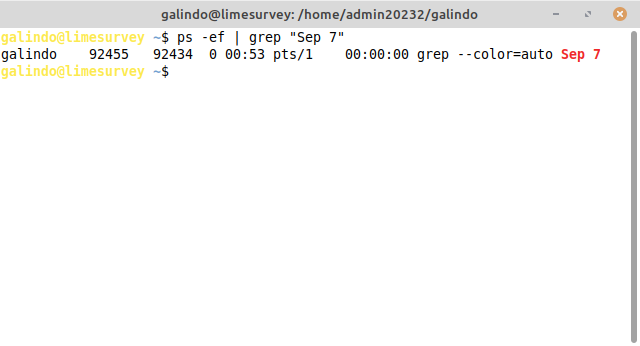
\includegraphics[width=10cm]{img/1.png}
\caption{Procesos iniciados el 7 de Septiembre}
\end{figure}

\begin{itemize}
\item \textbf{ps} Para mostrar los procesos del usuario:
\begin{itemize}
\item \textbf{-e} Lista información sobre cada proceso del sistema
\item \textbf{-f} muestra los detalle de los procesos
\end{itemize}

\item \textbf{grep} para buscar el string de la fecha
\end{itemize}

\pagebreak

\subsection{Qué están haciendo los procesos que actualmente esta ejecutando maestro. (Comando)}
\label{sec:org1ca9ef1}
\begin{verbatim}
ps -fu lety
\end{verbatim}

\begin{figure}[htbp]
\centering
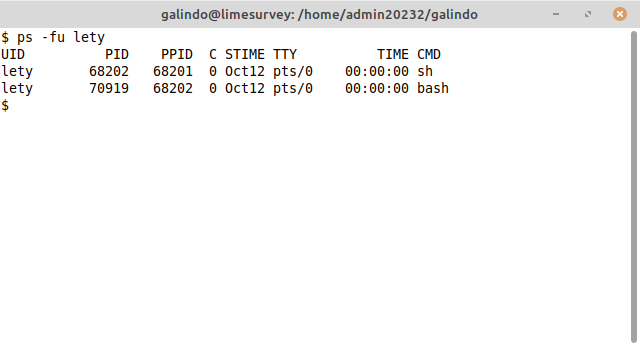
\includegraphics[width=9cm]{img/2.png}
\caption{Nada solo aparecen que tiene sh abierto}
\end{figure}

\subsection{Genere un listado con el número de proceso, número del proceso padre, comando en ejecución y prioridad de tres de sus compañeros.}
\label{sec:orgb3c0679}
\begin{verbatim}
ps -feao user,group,pid,ppid,cmd,nice | grep "admi*"
\end{verbatim}

\begin{description}
\item[{f}] Muestra una lista completa de procesos con detalles y usuario.
\item[{e}] Lista información sobre cada proceso en ejecución ahora.
\item[{a}] Muestra los procesos de otros usuarios.
\item[{o}] Muestra la información de acuerdo a un formato especificado.
\end{description}

\begin{figure}[htbp]
\centering
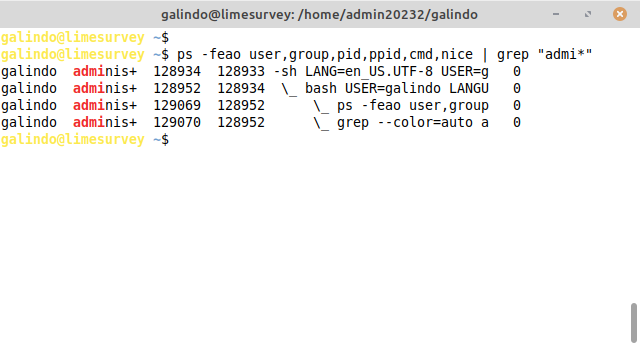
\includegraphics[width=10cm]{img/3.png}
\caption{Solo estoy yo en el servidor}
\end{figure}

\subsection{Explique la diferencia entre las opciones de ps e,f,l y j}
\label{sec:org7ef7970}

\begin{description}
\item[{e}] Lista información sobre cada proceso en ejecución ahora.
\item[{f}] Muestra una lista completa de procesos con detalles y usuario.
\item[{l}] Genera una lista con información detallada de los procesos.
\item[{j}] La información se presenta empezando por el PID
\end{description}

\subsection{Explique la diferencia entre las opciones de ps a y u}
\label{sec:orgfc817b9}
\begin{description}
\item[{a}] muestra los procesos de todos los usuarios.
\item[{u}] muestra procesos de un usuario específico.
\end{description}

\pagebreak

\subsection{Explique qué es lo que hace la opción de ps t y u Si tiene dos sesiones de ssh abiertas con el mismo user name}
\label{sec:org0059808}
\subsubsection*{Flag -t}
\label{sec:org96db1aa}
Lista los procesos asociados con la terminal. Por ejemplo, term/a, o pts/0, si
tenemos mas de una terminal y solo usamos \textbf{-t} mostrara los procesos de esa 
terminal.  

\begin{figure}[htbp]
\centering
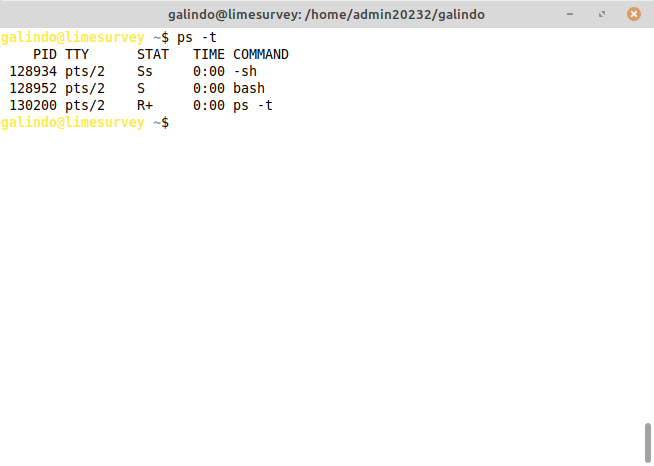
\includegraphics[width=10cm]{img/mt.png}
\caption{salida de ps -t}
\end{figure}

\subsubsection*{Flag -u}
\label{sec:orgc1a2b4b}
el usuario visualiza los procesos del usuario independientemente de la terminal
que use.

\begin{figure}[htbp]
\centering
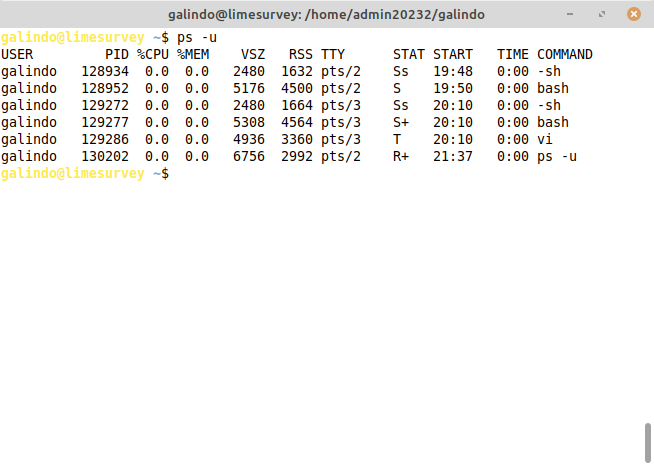
\includegraphics[width=10cm]{img/mu.png}
\caption{Salida de ps -u}
\end{figure}

\subsection{¿qué procesos muestra al ejecutar ps?}
\label{sec:org8bf8059}
El comando ps reporta el estado de los procesos activos

\begin{figure}[htbp]
\centering
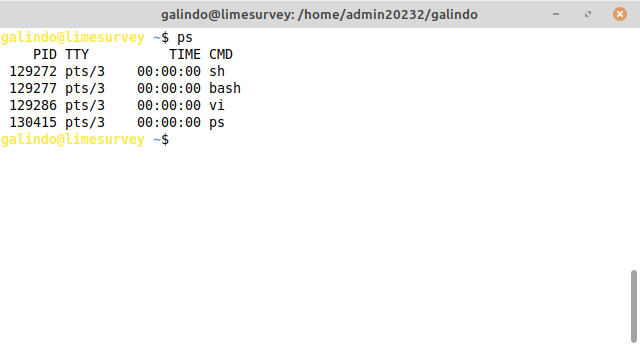
\includegraphics[width=10cm]{img/ps.png}
\caption{Procesos activos en mi usuario}
\end{figure}

\subsection{¿Qué opción de ps debería de usar par}
\label{sec:org26019ec}
a ver todos los procesos de un usuario?
\begin{verbatim}
ps -U <nombre del usuario>
\end{verbatim}

\begin{figure}[htbp]
\centering
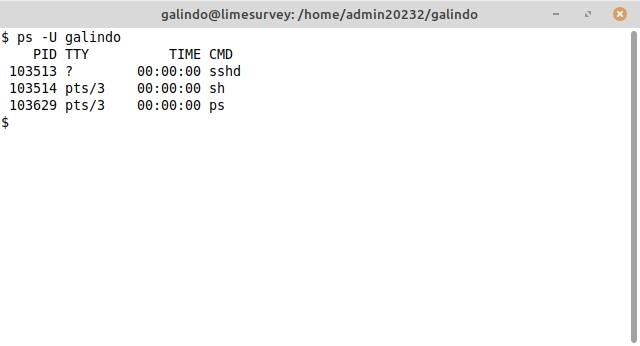
\includegraphics[width=10cm]{img/psmu.png}
\caption{Procesos activos en mi usuario}
\end{figure}
\pagebreak

\subsection{¿Cómo identifico a los procesos que el usuario está ejecutando en cada terminal?}
\label{sec:org5f32837}
\begin{itemize}
\item Utilizando la columna TTY en \texttt{ps -f} o tambien utilizando \texttt{ps -o tty,cmd}
\end{itemize}

\begin{figure}[htbp]
\centering
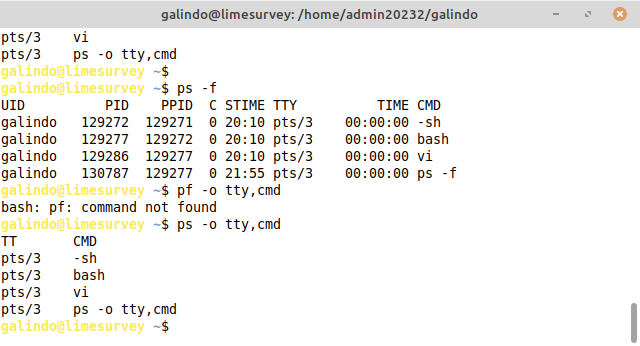
\includegraphics[width=10cm]{img/tty.png}
\caption{}
\end{figure}

\subsection{¿Cuál es significado de TODAS las columnas de formato que maneja ps –o? (Sólo las que no están explicadas en este material).}
\label{sec:org30d149b}
\autocite{ibm}
\begin{description}
\item[{ruser}] Indica el ID de usuario real del proceso. Se muestra el ID de usuario en formato de texto. Si no se puede obtener el ID de usuario en formato de texto, se utiliza una representación decimal. El encabezado predeterminado para este campo es RUSER.

\item[{rgroup}] Indica el ID de grupo real del proceso. Se muestra el ID de grupo en formato de texto. Si no se puede obtener el ID de grupo en formato de texto, se utiliza una representación decimal. El encabezado predeterminado para este campo es RGROUP.

\item[{ruid}] Indica el número de ID de usuario real del proceso en formato decimal. El encabezado predeterminado para este campo es RUID.

\item[{gid}] Indica el número de ID de grupo efectivo del proceso en formato decimal. El nombre de inicio de sesión se imprime bajo la opción -f.

\item[{rgid}] Indica el número de ID de grupo real del proceso en formato decimal. El encabezado predeterminado para este campo es RGID.

\item[{pid}] Indica el valor decimal del ID de proceso. El encabezado predeterminado para este campo es PID.

\item[{ppid}] Indica el valor decimal del ID de proceso principal (padre). El encabezado predeterminado para este campo es PPID.

\item[{pgid}] Indica el valor decimal del ID de grupo de procesos. El encabezado predeterminado para este campo es PGID.

\item[{sid}] Indica el ID de proceso del líder de sesión. El encabezado predeterminado para este campo es SID.

\item[{pcpu}] Indica la proporción de tiempo de CPU utilizado en relación al tiempo de CPU disponible, expresada como porcentaje. El encabezado predeterminado para este campo es \%CPU.

\item[{pmem}] Indica el porcentaje de memoria real utilizada por este proceso. El encabezado predeterminado para este campo es \%MEM.

\item[{vsz}] Indica, en formato decimal, el tamaño en kilobytes de la imagen base del núcleo del proceso. El encabezado predeterminado para este campo es VSZ.

\item[{rss}] (bandera v) El tamaño de memoria real (conjunto residente) del proceso (en unidades de 1 KB).

\item[{nice}] Indica el valor decimal del valor "nice" del proceso. El encabezado predeterminado para este campo es NI.

\item[{class}] Indica la política de programación para un hilo de kernel. Las políticas son sched\_other, sched\_fifo y sched\_rr. El encabezado predeterminado para este campo es CLS.

\item[{time}] Indica el tiempo acumulado de CPU desde que el proceso se inició. El tiempo se muestra en el mismo formato que en etime. El encabezado predeterminado para este campo es TIME.

\item[{etime}] Indica el tiempo transcurrido desde que el proceso se inició.

\item[{stime}] La hora de inicio del proceso. Las variables de entorno LANG controlan la apariencia de este campo.

\item[{lwp}] El tiempo de ejecución de un hilo de ejecución ligero individual.

\item[{nlwp}] Indica el número de hilos de kernel propiedad del proceso. El encabezado predeterminado para este campo es THCNT.

\item[{psr}] El número de procesador lógico al que está vinculado el hilo de kernel (si lo tiene). Para un proceso, este campo se muestra si todos sus hilos están vinculados al mismo procesador.

\item[{tty}] La terminal de control para el proceso.

\item[{addr}] Contiene el número de segmento de la pila del proceso, si es normal; si es un proceso de kernel, la dirección del área de datos previos al procesamiento.

\item[{wchan}] Indica el evento por el que el proceso o hilo de kernel está esperando o durmiendo. Para un hilo de kernel, este campo está en blanco si el hilo de kernel está en ejecución.

\item[{fname}] Indica los primeros 8 bytes del nombre base del archivo ejecutable del proceso. El encabezado predeterminado para este campo es COMMAND.

\item[{args}] Indica el nombre completo del comando que se está ejecutando. Se incluyen todos los argumentos de línea de comandos, aunque puede producirse truncamiento. El encabezado predeterminado para este campo es COMMAND.

\item[{project}] Nombre del proyecto asignado al proceso. En el entorno operativo actual, los campos PROJECT y USER no se traducen a nombres para los procesos que se ejecutan dentro de una partición de trabajo.
\end{description}

\subsection{Ejecute dos comandos en background (los que quiera).}
\label{sec:orgdc403e1}
\begin{verbatim}
nano&
vi&
\end{verbatim}

\begin{figure}[htbp]
\centering
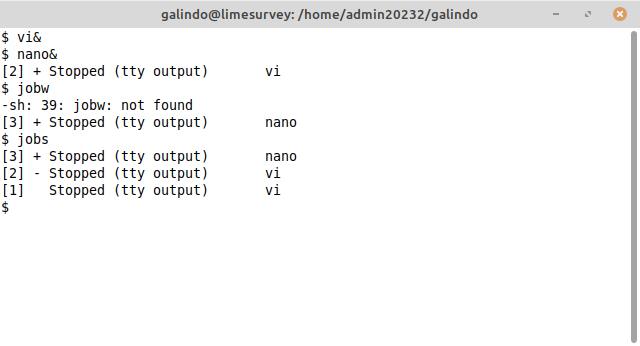
\includegraphics[width=10cm]{img/nanovi.png}
\caption{Nano y Vi corriendo en el fondo}
\end{figure}

\subsection{Ejecute el comando cat >lista, ¿Qué prioridad tiene asignada?}
\label{sec:orga6e32d9}
\begin{itemize}
\item Tiene la prioridad 19
\end{itemize}

\begin{figure}[htbp]
\centering
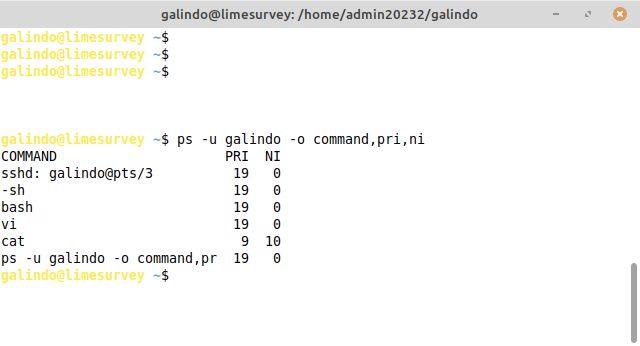
\includegraphics[width=10cm]{img/psprimi.png}
\caption{use ps desde otra terminal para ve la prioridad}
\end{figure}

\pagebreak

\subsection{Mate el proceso anterior.}
\label{sec:org6a72caf}
\begin{verbatim}
kill -9 130985
\end{verbatim}

\begin{figure}[htbp]
\centering
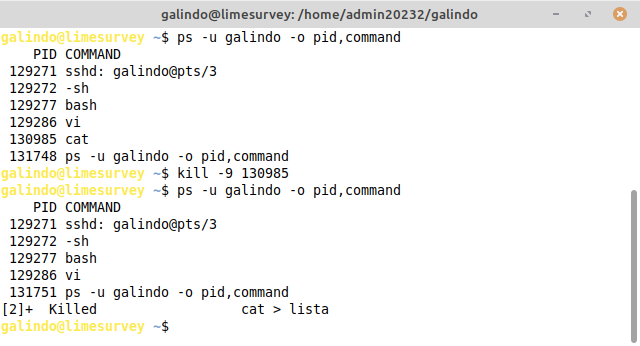
\includegraphics[width=10cm]{img/kill.png}
\caption{Matar el proceso}
\end{figure}

\subsection{Vuelva a ejecutar cat>lista pero con menor prioridad.}
\label{sec:org6d31ed7}
\begin{verbatim}
nice -n 10 cat>lista
\end{verbatim}

\begin{figure}[htbp]
\centering
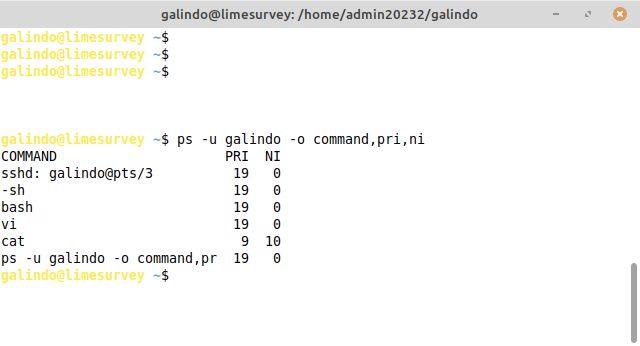
\includegraphics[width=10cm]{img/psprimi.png}
\caption{Nice ahora es mayor y la prioridad es mas baja}
\end{figure}

\subsubsection*{¿Qué prioridad le fue asignada?}
\label{sec:org7739010}
\begin{itemize}
\item Prioridad marca 9
\end{itemize}

\pagebreak

\subsection{Una vez más ejecute cat>lista, pero ahora en el background .}
\label{sec:orgf24ec62}
\begin{verbatim}
cat>list&
\end{verbatim}

\begin{figure}[htbp]
\centering
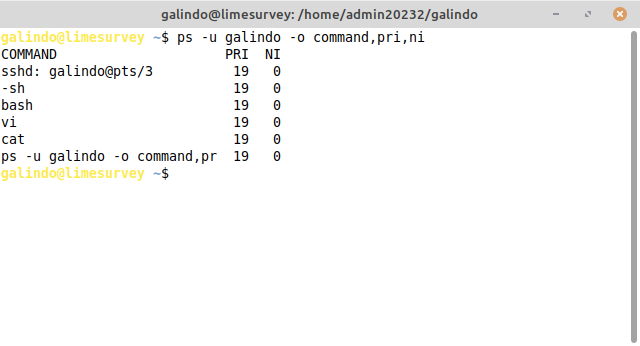
\includegraphics[width=10cm]{img/prioridad1.png}
\caption{salida de ps -u}
\end{figure}

\subsection{¿Cuál es su prioridad ahora?}
\label{sec:org505c7c8}
\begin{itemize}
\item El valor de prioridad es '19' y el valor de nice es '0'
\end{itemize}

\subsection{Verifique que el comando en background este en la lista de procesos.}
\label{sec:org99c47a9}
\begin{verbatim}
ps -l
\end{verbatim}

\begin{figure}[htbp]
\centering
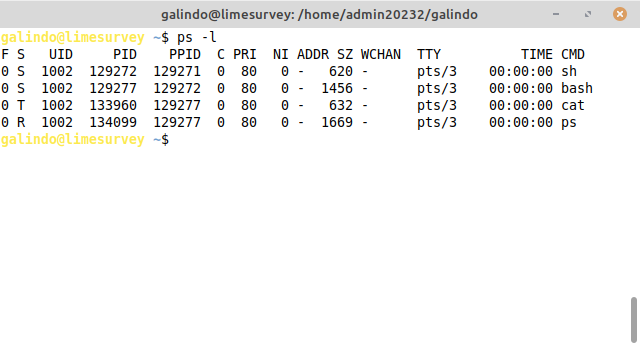
\includegraphics[width=10cm]{img/psml.png}
\caption{lista de procesos}
\end{figure}

\pagebreak

\subsection{Verifique que el comando en background este en la lista de tareas (jobs).}
\label{sec:org63cfd33}
\begin{verbatim}
jobs
\end{verbatim}

\begin{figure}[htbp]
\centering
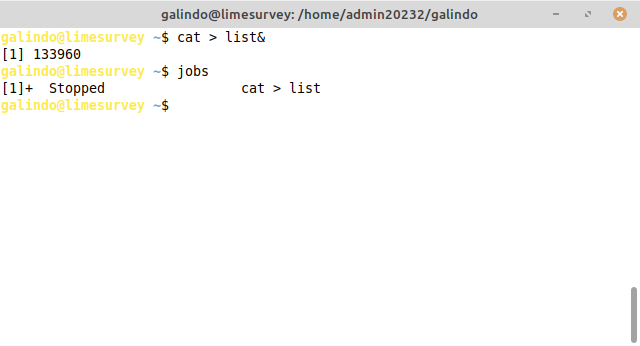
\includegraphics[width=10cm]{img/jobs.png}
\caption{Lista de tareas}
\end{figure}

\subsection{Pase una de las tareas al foreground (use el número de tarea)}
\label{sec:org6c1068c}
\begin{verbatim}
fg %1 
\end{verbatim}

\begin{figure}[htbp]
\centering
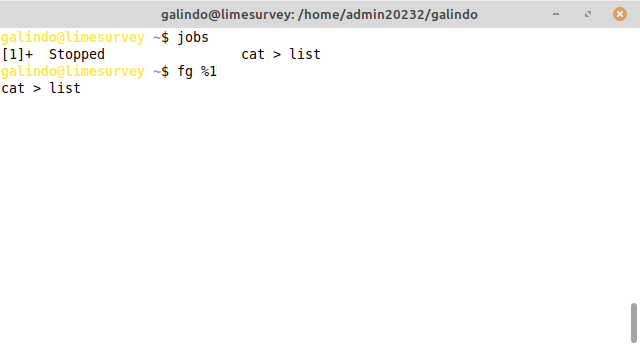
\includegraphics[width=10cm]{img/random.png}
\caption{traer el proceso '1' al foreground}
\end{figure}

\subsection{Pase la otra tarea al foreground, pero ahora use el número de PID.}
\label{sec:orgad44142}
\begin{itemize}
\item en este comando no se puede ejecutar en esta distribución
\end{itemize}

\subsection{Envíe otro comando al background.}
\label{sec:orge5c8d90}
\begin{verbatim}
vi&
\end{verbatim}

\subsection{Finalice este proceso.}
\label{sec:org3de0cac}
\begin{verbatim}
kill -9 134242
\end{verbatim}

\begin{figure}[htbp]
\centering
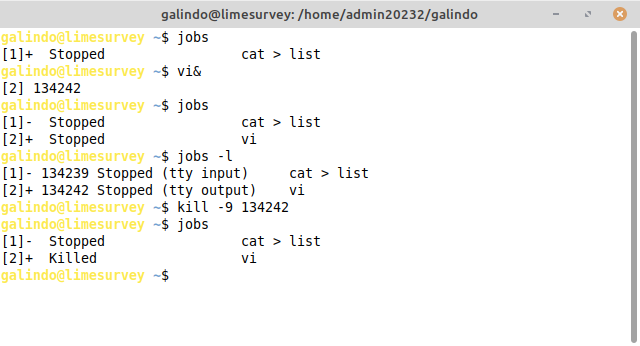
\includegraphics[width=10cm]{img/vi.png}
\caption{Proceso vi creado en el fondo y detenido}
\end{figure}

\section{Conclusión}
\label{sec:orgf66df9f}
Durante esta practica aprendi como crear procesos, como leer procesos y como usar 
comandos para mandar al fondo y trer de vuelta, siento que estos comandos me 
seran muy utiles para poder trabajar y no tener que estar haciendo scripts para
todo.

\section{Fuentes}
\label{sec:org2948f26}
\printbibliography[heading=none]
\end{document}
